\documentclass[12pt, a4paper]{article}\usepackage[]{graphicx}\usepackage[]{xcolor}
% maxwidth is the original width if it is less than linewidth
% otherwise use linewidth (to make sure the graphics do not exceed the margin)
\makeatletter
\def\maxwidth{ %
  \ifdim\Gin@nat@width>\linewidth
    \linewidth
  \else
    \Gin@nat@width
  \fi
}
\makeatother

\definecolor{fgcolor}{rgb}{0.345, 0.345, 0.345}
\newcommand{\hlnum}[1]{\textcolor[rgb]{0.686,0.059,0.569}{#1}}%
\newcommand{\hlstr}[1]{\textcolor[rgb]{0.192,0.494,0.8}{#1}}%
\newcommand{\hlcom}[1]{\textcolor[rgb]{0.678,0.584,0.686}{\textit{#1}}}%
\newcommand{\hlopt}[1]{\textcolor[rgb]{0,0,0}{#1}}%
\newcommand{\hlstd}[1]{\textcolor[rgb]{0.345,0.345,0.345}{#1}}%
\newcommand{\hlkwa}[1]{\textcolor[rgb]{0.161,0.373,0.58}{\textbf{#1}}}%
\newcommand{\hlkwb}[1]{\textcolor[rgb]{0.69,0.353,0.396}{#1}}%
\newcommand{\hlkwc}[1]{\textcolor[rgb]{0.333,0.667,0.333}{#1}}%
\newcommand{\hlkwd}[1]{\textcolor[rgb]{0.737,0.353,0.396}{\textbf{#1}}}%
\let\hlipl\hlkwb

\usepackage{framed}
\makeatletter
\newenvironment{kframe}{%
 \def\at@end@of@kframe{}%
 \ifinner\ifhmode%
  \def\at@end@of@kframe{\end{minipage}}%
  \begin{minipage}{\columnwidth}%
 \fi\fi%
 \def\FrameCommand##1{\hskip\@totalleftmargin \hskip-\fboxsep
 \colorbox{shadecolor}{##1}\hskip-\fboxsep
     % There is no \\@totalrightmargin, so:
     \hskip-\linewidth \hskip-\@totalleftmargin \hskip\columnwidth}%
 \MakeFramed {\advance\hsize-\width
   \@totalleftmargin\z@ \linewidth\hsize
   \@setminipage}}%
 {\par\unskip\endMakeFramed%
 \at@end@of@kframe}
\makeatother

\definecolor{shadecolor}{rgb}{.97, .97, .97}
\definecolor{messagecolor}{rgb}{0, 0, 0}
\definecolor{warningcolor}{rgb}{1, 0, 1}
\definecolor{errorcolor}{rgb}{1, 0, 0}
\newenvironment{knitrout}{}{} % an empty environment to be redefined in TeX

\usepackage{alltt}

%%%%%%%%%%%%%%%%%%%%%%%%%%%%%%%%%%%%%%%%%%%%%%%%%%%%%%%%%%%%%%%%
% additional LaTeX packages
\usepackage[utf8]{inputenc}
\usepackage[top=2.5cm, bottom=2.5cm, left=2cm, right=2cm]{geometry}
\usepackage{graphicx}
\usepackage{float}
\usepackage[colorlinks=true, linkcolor=blue]{hyperref}
\usepackage{amsmath}

%%%%%%%%%%%%%%%%%%%%%%%%%%%%%%%%%%%%%%%%%%%%%%%%%%%%%%%%%%%%%%%%

% global settings


\IfFileExists{upquote.sty}{\usepackage{upquote}}{}
\begin{document}

%%%%%%%%%%%%%%%%%%%%%%%%%%%%%%%%%%%%%%%%%%%%%%%%%%%%%%%%%%%%%%%%
\title{Advanced Applications of Statistical Packages\\Report 2: Bootstrap Methods}
\author{Dawid Rurzyński, Samanta Szenajch}
\maketitle

\tableofcontents
\newpage

%%%%%%%%%%%%%%%%%%%%%%%%%%%%%%%%%%%%%%%%%%%%%%%%%%%%%%%%%%%%%%%%
\section{Task 1: Monte Carlo Simulations - ML vs Bootstrap}
%%%%%%%%%%%%%%%%%%%%%%%%%%%%%%%%%%%%%%%%%%%%%%%%%%%%%%%%%%%%%%%%

\subsection{Overview}

We compared maximum likelihood (ML) and bootstrap mean estimators for Gamma distribution parameters using Monte Carlo simulations with 1,000 iterations and 10,000 bootstrap resamples per sample.

\textbf{Gamma distribution parametrization:} We use the shape-scale parametrization where $X \sim \text{Gamma}(\alpha, \beta)$, with $\alpha$ being the shape parameter and $\beta$ the scale parameter. Three parameter pairs were tested: $\theta=(0.5,1)$, $(10,1)$, and $(10,3)$, representing different skewness levels. Sample sizes were $n=20, 50, 200$, resulting in 9 scenarios total.

\subsection{Results}

\begin{knitrout}
\definecolor{shadecolor}{rgb}{0.969, 0.969, 0.969}\color{fgcolor}\begin{kframe}
\begin{verbatim}
## 
## Task 1 Results Summary (all sample sizes and theta parameters):
## 
##        n theta_pair param true_value mean_theta_ml mean_theta_bs coverage
##   n = 20   (0.5, 1) alpha        0.5        0.5535        0.6235      87%
##   n = 20   (0.5, 1)  beta        1.0        0.9883        0.9463    84.7%
##   n = 20    (10, 1) alpha       10.0       11.9924       13.9999    80.3%
##   n = 20    (10, 1)  beta        1.0        0.9285        0.8822    80.8%
##   n = 20    (10, 3) alpha       10.0       11.5119       13.4542    84.2%
##   n = 20    (10, 3)  beta        3.0        2.8979        2.7537      84%
##   n = 50   (0.5, 1) alpha        0.5        0.5236        0.5471    90.5%
##   n = 50   (0.5, 1)  beta        1.0        0.9903        0.9738      87%
##   n = 50    (10, 1) alpha       10.0       10.6973       11.3426    86.8%
##   n = 50    (10, 1)  beta        1.0        0.9745        0.9550    86.8%
##   n = 50    (10, 3) alpha       10.0       10.5888       11.2361    89.4%
##   n = 50    (10, 3)  beta        3.0        2.9567        2.8976    89.5%
##  n = 200   (0.5, 1) alpha        0.5        0.5042        0.5097    92.9%
##  n = 200   (0.5, 1)  beta        1.0        0.9969        0.9929    93.1%
##  n = 200    (10, 1) alpha       10.0       10.1371       10.2881    93.7%
##  n = 200    (10, 1)  beta        1.0        0.9966        0.9916      94%
##  n = 200    (10, 3) alpha       10.0       10.1365       10.2855    93.9%
##  n = 200    (10, 3)  beta        3.0        2.9867        2.9718    93.5%
\end{verbatim}
\end{kframe}
\end{knitrout}

The column \texttt{true\_value} denotes the true value of the parameter reported in a given row: $\alpha$ for rows labelled \texttt{alpha} and $\beta$ for rows labelled \texttt{beta}.

\subsubsection{Normality Assessment}

Bootstrap distributions of MLE estimates were assessed using histogram and Q-Q plot diagnostics together with Shapiro-Wilk normality tests. For small samples ($n=20$), bootstrap estimates show visible skewness and deviations from normality, especially for highly skewed parameters such as $\theta=(0.5,1)$. For larger samples ($n=200$), the distributions become closer to a bell-shaped form, but small systematic deviations remain visible in the Q-Q plots.

\textbf{Can we assume normality?} Formal Shapiro-Wilk tests reject normality in all scenarios. Graphically, the bootstrap distributions become closer to normal for larger samples, especially for $n=200$, but normality should not be assumed without caution. Therefore, bootstrap confidence intervals are preferred over relying only on normal-theory approximations.

\subsubsection{Graphical Diagnostics}

Histogram and Q-Q plot pairs were generated for all 9 scenarios and both parameters $\alpha$ and $\beta$, giving 18 diagnostic panels in total. These plots were used as graphical diagnostics for assessing the shape of the bootstrap distributions. Two representative examples are shown below: one for a small-sample, skewed case and one for a larger-sample case.

\begin{figure}[H]
\centering
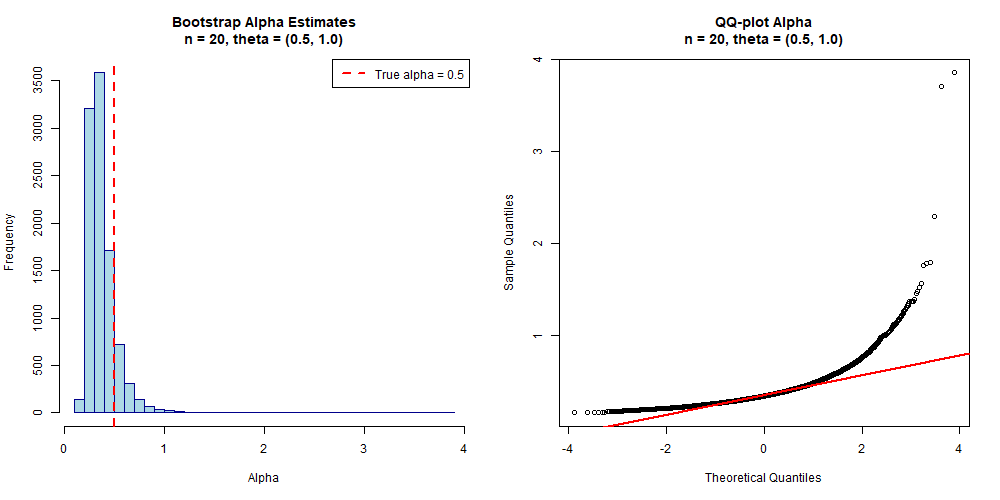
\includegraphics[width=0.92\textwidth]{figure/task1_hist_qq_alpha_n20_theta1.png}
\caption{Bootstrap distribution and Q-Q plot for $\alpha$, $n=20$, $\theta=(0.5,1)$. The bootstrap distribution is visibly skewed, so normality is not a reasonable assumption in this case.}
\label{fig:task1_alpha_n20}
\end{figure}

\begin{figure}[H]
\centering
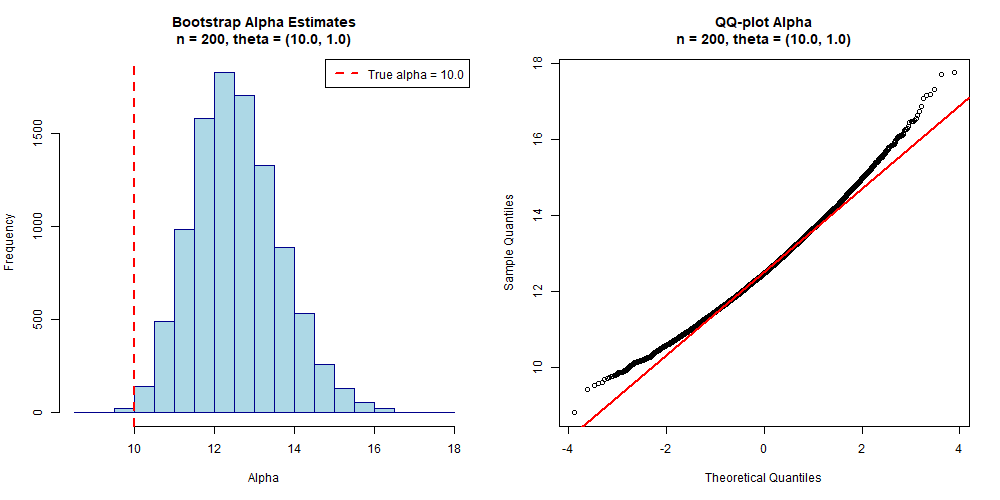
\includegraphics[width=0.92\textwidth]{figure/task1_hist_qq_alpha_n200_theta2.png}
\caption{Bootstrap distribution and Q-Q plot for $\alpha$, $n=200$, $\theta=(10,1)$. The distribution is closer to normal than in the small-sample case, but small deviations remain.}
\label{fig:task1_alpha_n200}
\end{figure}

\subsubsection{Shapiro-Wilk Normality Tests}

Shapiro-Wilk tests were performed on random subsets of 5000 bootstrap estimates, because the R implementation of the test does not allow samples larger than 5000 observations. The full results are saved in \texttt{results/task1\_normality\_tests.rds}. The table below reports the final numerical results.

\begin{center}
\small
\begin{tabular}{ccccc}
\hline
$n$ & $\theta$ & Parameter & Shapiro-Wilk $p$-value & Conclusion \\
\hline
20 & $(0.5,1)$ & $\alpha$ & 1.33e-65 & Evidence against \\
20 & $(0.5,1)$ & $\beta$ & 1.15e-24 & Evidence against \\
20 & $(10,1)$ & $\alpha$ & 1.48e-52 & Evidence against \\
20 & $(10,1)$ & $\beta$ & 8.69e-17 & Evidence against \\
20 & $(10,3)$ & $\alpha$ & 2.46e-56 & Evidence against \\
20 & $(10,3)$ & $\beta$ & 5.85e-25 & Evidence against \\
50 & $(0.5,1)$ & $\alpha$ & 3.30e-34 & Evidence against \\
50 & $(0.5,1)$ & $\beta$ & 1.11e-22 & Evidence against \\
50 & $(10,1)$ & $\alpha$ & 2.74e-36 & Evidence against \\
50 & $(10,1)$ & $\beta$ & 4.01e-21 & Evidence against \\
50 & $(10,3)$ & $\alpha$ & 5.36e-39 & Evidence against \\
50 & $(10,3)$ & $\beta$ & 1.13e-08 & Evidence against \\
200 & $(0.5,1)$ & $\alpha$ & 1.70e-17 & Evidence against \\
200 & $(0.5,1)$ & $\beta$ & 2.86e-09 & Evidence against \\
200 & $(10,1)$ & $\alpha$ & 6.59e-16 & Evidence against \\
200 & $(10,1)$ & $\beta$ & 0.0165 & Evidence against \\
200 & $(10,3)$ & $\alpha$ & 4.67e-18 & Evidence against \\
200 & $(10,3)$ & $\beta$ & 1.15e-06 & Evidence against \\
\hline
\end{tabular}
\end{center}


Because the Shapiro-Wilk test is very sensitive for large samples, the conclusions were based jointly on $p$-values, histograms, and Q-Q plots. The tests formally reject normality in all scenarios, although the graphical diagnostics show that the bootstrap distributions become closer to normal as $n$ increases.

\subsubsection{Key Findings}

\begin{itemize}
\item \textbf{ML vs Bootstrap:} Across all simulated scenarios, the maximum likelihood estimator generally achieved smaller mean absolute error than the bootstrap mean estimator. This difference was most pronounced for smaller samples ($n=20$). For $n=200$, both estimators converged closer to the true parameters, with ML maintaining a slight advantage.

\item \textbf{Coverage:} Bootstrap confidence intervals achieved 80--94\% coverage across scenarios. Coverage was below the nominal 95\% level, especially for $n=20$ and highly skewed parameters. For $n=200$, coverage improved to approximately 93--94\%, approaching the nominal level more closely. The undercoverage is most visible for small samples and skewed Gamma distributions, which is expected because the bootstrap approximation is less stable in such cases.

\item \textbf{Normality:} Shapiro-Wilk tests formally rejected normality for all bootstrap distributions. However, graphical diagnostics showed that deviations from normality were strongest for $n=20$ and skewed Gamma distributions, while distributions for $n=200$ were closer to normal. Therefore, normal approximation should be treated cautiously and supported by bootstrap-based inference.
\end{itemize}

\textbf{Overall:} Normality cannot be assumed for all bootstrap distributions. The normal approximation is especially questionable for $n = 20$ and skewed Gamma distributions. For $n = 200$, bootstrap distributions are closer to normal, but the assessment still supports using bootstrap confidence intervals rather than relying only on normal-theory approximations.

%%%%%%%%%%%%%%%%%%%%%%%%%%%%%%%%%%%%%%%%%%%%%%%%%%%%%%%%%%%%%%%%
\section{Task 2: Bootstrap Confidence Intervals for R-squared}
%%%%%%%%%%%%%%%%%%%%%%%%%%%%%%%%%%%%%%%%%%%%%%%%%%%%%%%%%%%%%%%%

\subsection{Problem}

We analyzed regression model $\log(\text{body}) \sim \log(\text{brain})$ using Animals dataset. Bootstrap method (10,000 resamples) computed 95\% confidence interval for $R^2$.

\subsection{Results}

\begin{knitrout}
\definecolor{shadecolor}{rgb}{0.969, 0.969, 0.969}\color{fgcolor}\begin{kframe}
\begin{verbatim}
## Sample size: 28
## Original R2: 0.6076
## Bootstrap mean: 0.6128
## Bootstrap bias: 0.005182
## 95% CI: [ 0.3004 , 0.9198 ]
\end{verbatim}
\end{kframe}
\end{knitrout}

\begin{figure}[H]
\centering
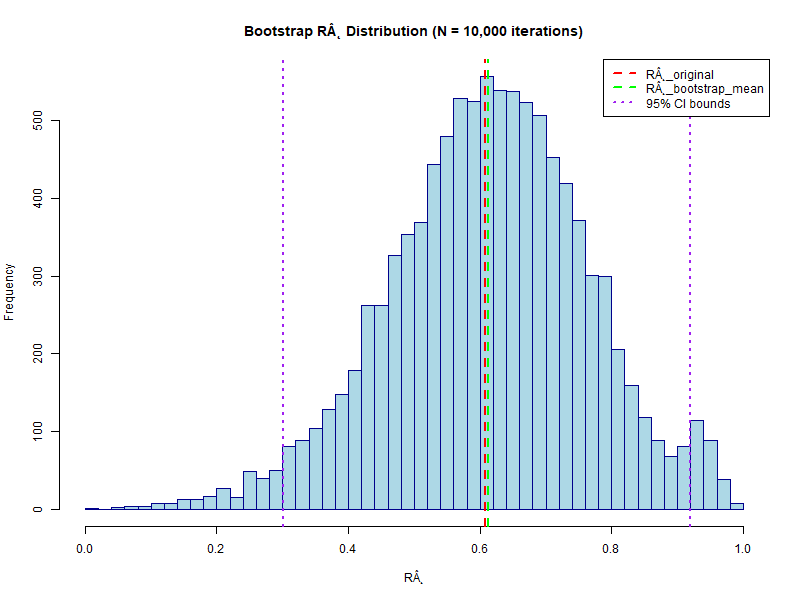
\includegraphics[width=0.7\textwidth]{figure/task2_histogram.png}
\caption{Bootstrap distribution of $R^2$ estimates (10,000 resamples). Original estimate shown as vertical line.}
\label{fig:task2}
\end{figure}

\subsubsection{Interpretation}

The bootstrap bias is small, but the 95\% confidence interval is relatively wide ($\approx 0.62$), indicating considerable uncertainty in the $R^2$ estimate. This wide interval reflects sampling variability and suggests caution in interpreting the model's predictive power as fixed across similar datasets.

%%%%%%%%%%%%%%%%%%%%%%%%%%%%%%%%%%%%%%%%%%%%%%%%%%%%%%%%%%%%%%%%
\section{Task 3: Salary Analysis - Married vs Unmarried}
%%%%%%%%%%%%%%%%%%%%%%%%%%%%%%%%%%%%%%%%%%%%%%%%%%%%%%%%%%%%%%%%

\subsection{Problem}

Bootstrap analysis (stratified by marital status, 10,000 resamples) of NBA player salaries with comparison of means and medians between married and unmarried players. Salary is measured in thousands of USD.

\subsection{Results}

\begin{knitrout}
\definecolor{shadecolor}{rgb}{0.969, 0.969, 0.969}\color{fgcolor}\begin{kframe}
\begin{verbatim}
## 
## === MEAN SALARY ANALYSIS ===
## 
## WHOLE SAMPLE:
##   Mean: $ 1423.83 K (95% CI: [ 1306.62 ,  1542.63 ])
## 
## MARRIED PLAYERS (n= 119 ):
##   Mean: $ 1600.98 K (95% CI: [ 1408.94 ,  1797.07 ])
## 
## UNMARRIED PLAYERS (n= 150 ):
##   Mean: $ 1283.29 K (95% CI: [ 1141.75 ,  1432.07 ])
## 
## DIFFERENCE IN MEANS (married - unmarried):
##   Point estimate: $ 317.69 K
##   95% CI: [ 80.32 ,  567.85 ]
##   Conclusion: Evidence of difference 
## 
## === MEDIAN SALARY ANALYSIS ===
## 
## WHOLE SAMPLE:
##   Median: $ 1186.00 K (95% CI: [ 1065.00 ,  1275.00 ])
## 
## MARRIED PLAYERS:
##   Median: $ 1275.00 K (95% CI: [ 1100.00 ,  1690.00 ])
## 
## UNMARRIED PLAYERS:
##   Median: $ 1091.25 K (95% CI: [ 884.00 ,  1226.50 ])
## 
## DIFFERENCE IN MEDIANS (married - unmarried):
##   Point estimate: $ 183.75 K
##   95% CI: [ -36.00 ,  659.98 ]
##   Conclusion: No evidence of difference
\end{verbatim}
\end{kframe}
\end{knitrout}

\begin{figure}[H]
\centering
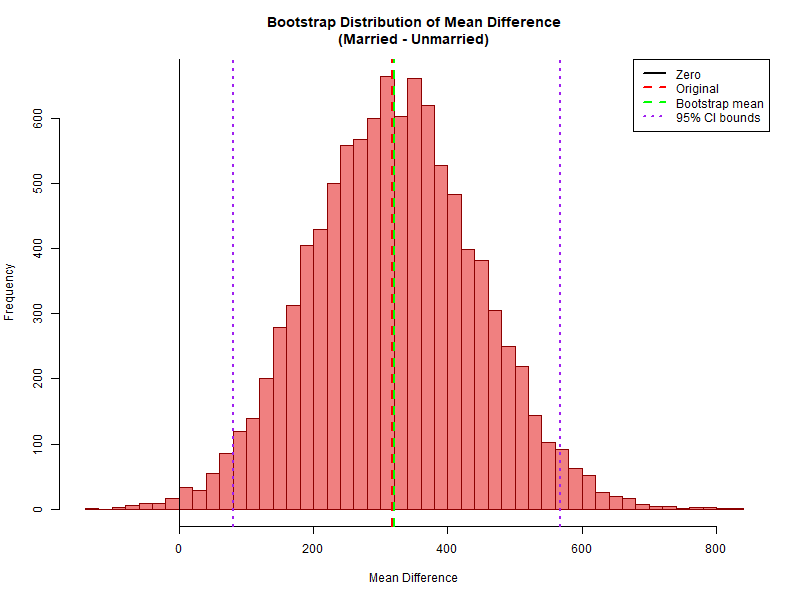
\includegraphics[width=0.7\textwidth]{figure/task3_diff_mean.png}
\caption{Bootstrap distribution of mean wage difference (married - unmarried). Vertical line at 0 reference.}
\label{fig:task3}
\end{figure}

\subsubsection{Interpretation}

\textbf{Mean salary:} The confidence interval for the mean difference does not contain zero, suggesting bootstrap evidence of higher mean salaries among married players (difference $\approx \$318$K). However, the result should be interpreted cautiously, as marital status may be associated with confounding factors such as player experience, age, or career stage.

\textbf{Median salary:} The bootstrap confidence interval for the median difference contains zero, so the data do not provide clear evidence of a difference in median salaries between married and unmarried players. This contrasts with the mean analysis, suggesting that the mean difference may be influenced by higher-earning players rather than by a clear shift in the typical salary level.

%%%%%%%%%%%%%%%%%%%%%%%%%%%%%%%%%%%%%%%%%%%%%%%%%%%%%%%%%%%%%%%%
\section{Task 4: Bootstrap Confidence Areas for L$_3$ Lorenz Curves}
%%%%%%%%%%%%%%%%%%%%%%%%%%%%%%%%%%%%%%%%%%%%%%%%%%%%%%%%%%%%%%%%

\subsection{Problem}

For quantile function $Q$, we estimated the curve $L_3(p; Q) = \frac{p^2 Q(p/2)}{Q(p/2) + Q(1-p/2)}$ using bootstrap with pointwise confidence areas.

\subsubsection{Part 1: Gamma Distribution}

Synthetic data generated from $\text{Gamma}(\alpha=2, \beta=4)$ with $n=60$. Bootstrap constructed pointwise 95\% confidence areas from 10,000 resamples.

\subsubsection{Part 2: NBA Salary Data}

Stratified bootstrap comparison of L$_3$ curves for married vs unmarried players.

\subsection{Results}

\begin{knitrout}
\definecolor{shadecolor}{rgb}{0.969, 0.969, 0.969}\color{fgcolor}\begin{kframe}
\begin{verbatim}
## PART 1 - Gamma Distribution:
## Sample size: 60 
## True L3 inside CI at all p values: YES (100%)
## 
## PART 2 - NBA Salary Data:
## Married players: 119 
## Unmarried players: 150 
## CI overlap percentage: 100.0% 
## Mean distance between curves: 0.0055
\end{verbatim}
\end{kframe}
\end{knitrout}

\begin{figure}[H]
\centering
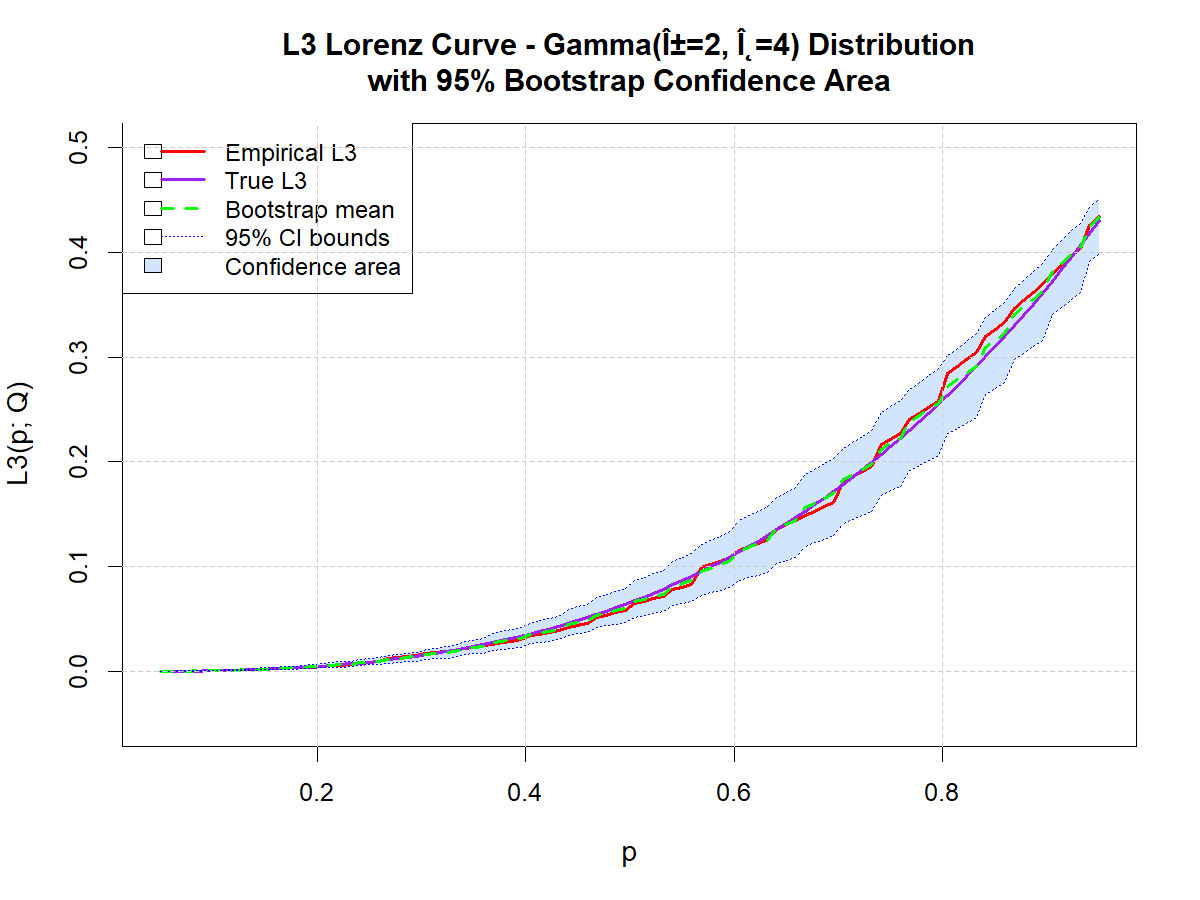
\includegraphics[width=0.8\textwidth]{figure/task4_part1_gamma.png}
\caption{L$_3$ Lorenz curve with bootstrap confidence area -- Gamma distribution. True curve (red) lies entirely within confidence bounds.}
\label{fig:task4a}
\end{figure}

\begin{figure}[H]
\centering
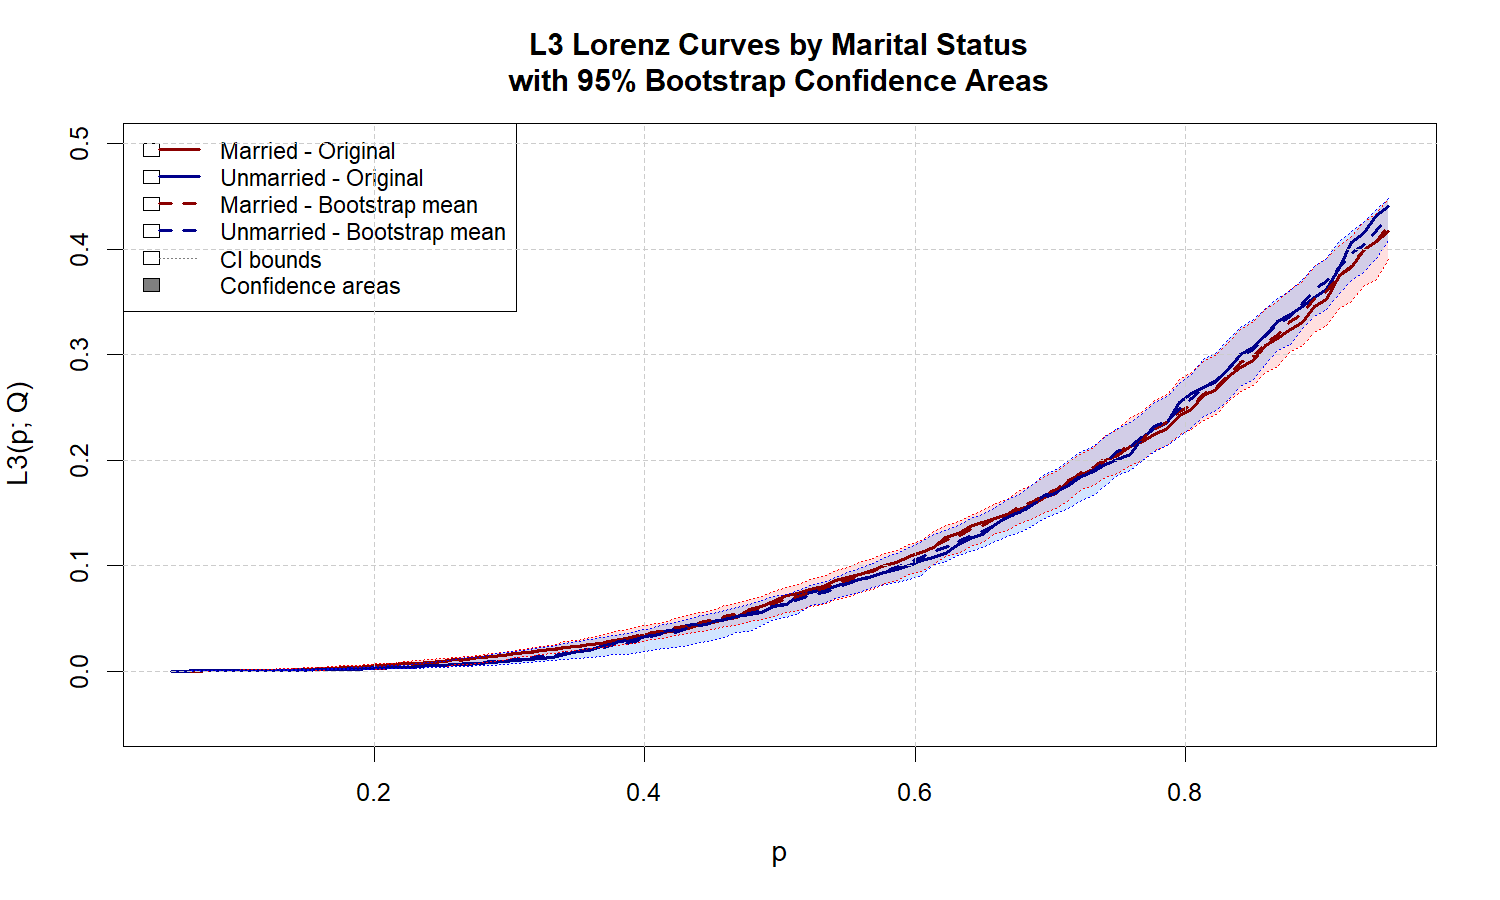
\includegraphics[width=0.8\textwidth]{figure/task4_part2_wage.png}
\caption{L$_3$ Lorenz curves by marital status -- NBA salaries. Confidence areas (shaded regions) for married (red) and unmarried (blue) players show substantial overlap.}
\label{fig:task4b}
\end{figure}

\subsubsection{Findings}

\textbf{Gamma distribution:} For the Gamma sample, the theoretical $L_3$ curve lies inside the pointwise bootstrap confidence area at all 100 evaluated $p$ values. This indicates that, in this simulation, the bootstrap confidence area captured the true curve well.

\textbf{NBA salary comparison:} The bootstrap confidence areas for married and unmarried players overlap across all evaluated $p$ values. This suggests similar $L_3$ curve shapes and thus similar structural properties of salary distributions across marital status groups. However, pointwise confidence areas are descriptive and should not be interpreted as formal simultaneous confidence bands or as formal evidence of distribution equality.

%%%%%%%%%%%%%%%%%%%%%%%%%%%%%%%%%%%%%%%%%%%%%%%%%%%%%%%%%%%%%%%%
\section{Summary}
%%%%%%%%%%%%%%%%%%%%%%%%%%%%%%%%%%%%%%%%%%%%%%%%%%%%%%%%%%%%%%%%

This report demonstrates bootstrap methodology applied to four distinct statistical problems: (1) Monte Carlo comparison of parameter estimators, (2) regression model inference, (3) group comparison with stratified bootstrap, and (4) curve estimation with confidence areas.

All analyses used 10,000 bootstrap resamples with 95\% confidence level. The results illustrate how bootstrap methods can be used for parameter estimation, model assessment, group comparisons, and curve estimation. However, some results indicate that bootstrap confidence intervals may deviate from nominal 95\% coverage, especially for small samples or complex statistics. For curve comparisons in Task 4, the confidence areas are pointwise and descriptive, not a formal global hypothesis test. The strongest limitations appear in small-sample bootstrap coverage (Task 1) and in the interpretation of pointwise confidence areas, which should not be treated as simultaneous confidence bands. Users should interpret all results with appropriate caution and consider context-specific assumptions.

\end{document}
